\chapter{Immersive Environments: XR in Composition}
\label{ch:xr-mus}

%\textbf{Question three (Shahrokh Yadegari):} once a spatial work is created and recorded, what open XR technologies exist that one can leverage to present their works?

%What are the technical difficulties associated with this kind of work? What are the artistic difficulties associated with this kind of work? 

%What are the differences between WebXR, MobileXR and HMDs (or related technologies like CAVEs)? Be able to talk about the visual system in relation to XR.

%critical lens  
%This chapter will be developed with Shahrokh Yadegari. 

In this chapter we will discuss how open-source developments in XR are allowing more composers to experiment with spatial music and how these multi-sensory systems might be leveraged in the future for the dissemination of their music. We will also discuss some of the new compositional techniques that systems of this sort allow: non-linear sequences, interactivity in general, gamification of musical material, etc. 

We will address the different open source frameworks available for the development of these experiences and the technical, and artistic, difficulties associated with these works. We will describe in detail the most popular systems available today for the development of XR experiences and discuss the differences between them in terms of their affordances and limitations.

Namely, we will discuss outline the key trade-offs between presenting spatial music using: HMDs, CAVEs, in concert halls, in gallery spaces, or any other modalities that we might encounter. We are interested in open systems, and especially those that are accessible to those with limited resources (ie. people outside university settings). Finally, we will address some of the fundamental philosophical implications of these systems as they relate to the dichotomy between performer, composer, and audience. 

\section{The History of VR}
The idea behind Virtual Reality (VR) can be argued to date back to the 1800s. In 1838, the first stereoscope was invented by Charles Wheatstone \cite{hemstrom2020comparison}. A stereoscope is a device in which a pair of images is presented to each eye in order to provide the illusion of depth. In 1965, Ivan Sutherland introduce the concept of "The Ultimate Display", which he described as: "a room within which the computer can control the existence of matter." \cite{sutherland1965ultimate} A few years later, Sutherland and his team would build "The Sword of Damocles", regarded today as the first VR head-mounted display (HMD).

\begin{figure}[ht!]%force figure here, top, strict
\centering
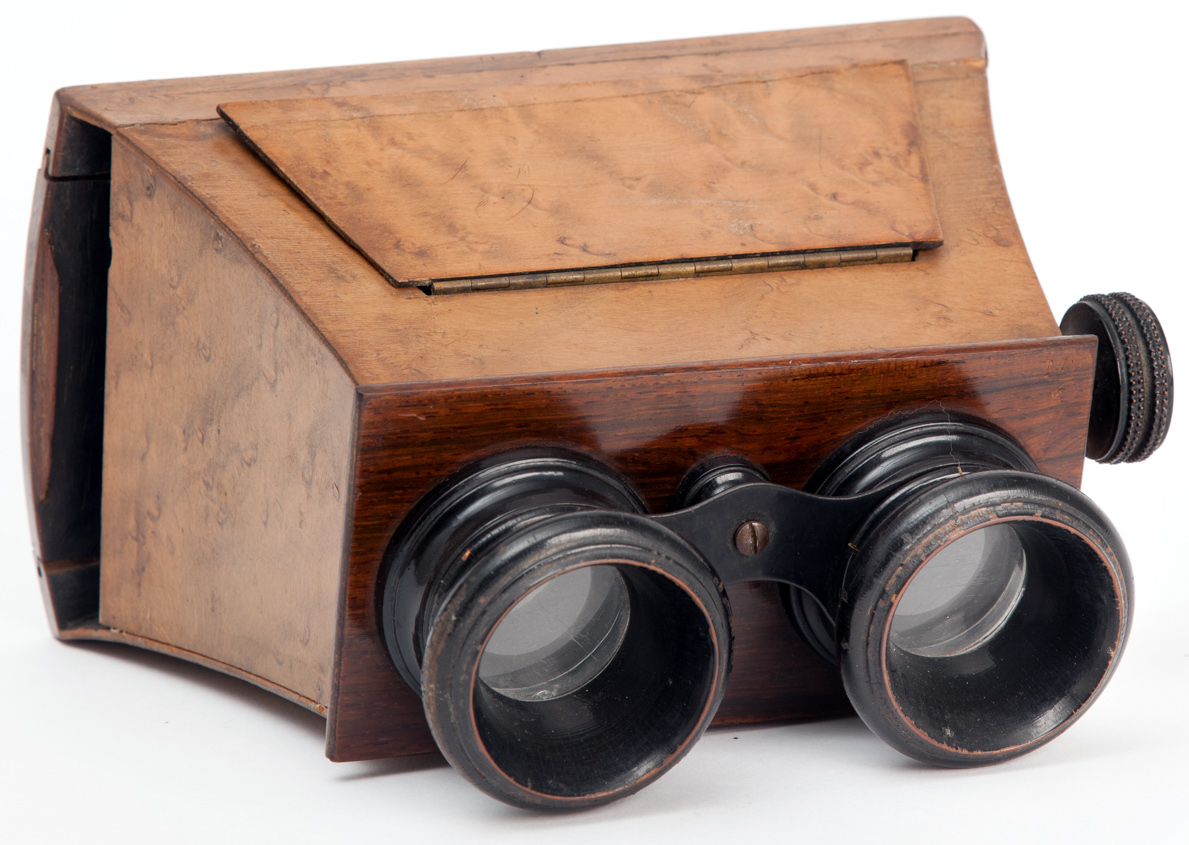
\includegraphics[width=0.7\textwidth]{img/stereoscope.jpg} 
%\captionsetup{justification=centering}
\caption{Brewster-type\protect\footnotemark stereoscope, 1870 \cite{FileIGB032online}}
\end{figure}

\footnotetext{Sir David Brewster (11 December 1781 – 10 February 1868) was a Scottish scientist, inventor, author, and academic administrator.}


\section{Contemporary XR Techniques}

\subsection{Hardware}
Inn this section we will discuss some of the popular hardware solutions that exist for creation and reproduction of XR content. 

\subsubsection{HMDs}
Head mounted displays.
%https://scholar.google.com/scholar?hl=en&as_sdt=0%2C5&q=head-mounted+display+ieee&btnG=

\subsubsection{MOCAP}
MOtion CAPture systems. 
%https://arxiv.org/pdf/1607.02046.pdf

\subsubsection{360\textdegree cameras}
% https://ieeexplore.ieee.org/stamp/stamp.jsp?arnumber=7892229&casa_token=GSr2i72N1-cAAAAA:RmRLZa4onN2qE6AMEd_Hg_0m_JcehUXB1J28wL6PzpUA89UV3ZoNXvsUqlWV5ZNHG8tF-j8Lcuzn&tag=1

\subsubsection{CAVEs}
%https://www.sciencedirect.com/science/article/pii/S0167739X08001167?casa_token=pOdchEnz0b0AAAAA:_5pB4ufLKxGIrH6Si-_Z3cy31P9H2ZkxIUAHbYxPW26c4rvBZhCQVLYyDcUiBFL9Ug5TZHll5-Fc

\section{Software}
\subsection{Game Engines}
Unity, Unreal, Godot, etc.

\subsection{WebXR}
% https://immersive-web.github.io/webxr-samples/explainer.html
%https://www.khronos.org/gltf/

% Most usage of WebGL today happens via frameworks that significantly simplify the creation of 3D scenes compared to using raw WebGL. Some of the more popular examples are three.js, babylon.js, and PlayCanvas. There's also frameworks that are specifically designed to create XR content on the web, such as A-Frame and ReactVR. These are all fantastic libraries with their own strengths and focuses, and in general it's recommended that you find tools that suit your needs and rely on them rather than trying to build your own rendering systems from scratch.

% However, most frameworks will also hide away the details of interacting with the WebXR API. That's generally great for users, but not terribly useful when the entire point of your code is to demonstrate how to use the API! At the same time, we don't want the WebXR logic to be obscured by hundreds of lines of WebGL calls. As a result, these samples make use of their own minimalistic rendering library that is specifically designed to highlight use of the WebXR API and de-emphasize the WebGL rendering logic. It is not recommended that you use this library in your own projects, as you will almost certainly be better served by one of the more popular, better established frameworks.

\subsection{Mobile XR}
\section{Open XR Tools }
\section{The Future of XR}
\section{Conclusion}



